\chapter{\label{chap:chap4} Validações}


Este capítulo abordará temas relacionados as validações realizadas neste projeto.
Sendo assim, nas seções a seguir serão apresentados temas como ambientes de simulações, cenários de testes e, por fim, estudos de casos


\section{Ambiente de simulação}

Em um primeiro momento a névoa foi construída de forma simulada utilizando a ferramenta Common Open Research Emulator (CORE)\cite{coregui}.
Para os primeiros experimentos a ferramente obteve resultados satisfatórios, porém quando foi necessário escalarmos a solução ela se mostrou ineficiente.
A ineficiência estava na criação dos nodos e na execução dos protocolos CoAP e Resource Mapping, uma vez que eles deveriam ser executados em todos os hosts da rede e não havia 
meios de automatizar este processo.

Esta automatização foi implantada utilizando a SDK de gerenciamento de containers Docker para Python, desta forma, foi possível criarmos névoas com tamanhos arbitrários
e, portanto, a ascalabilidade da solução pode ser amplamente testada\cite{dockersdk:2018}.

Cabe ressaltar que containers Docker\cite{docker:2018} consomem recursos da máquina hospedeira, tais como memória, processamento e disco rígido.
Portanto, a criação de instâncias de nodos (executando em containers) está limitada à quantidade de memória e capacidade de processamento da máquina hospedeira.


Cada container executa uma distrbuição Linux chamada Alpine, de aproximadamente 5Mb, que possui apenas as funcioalidades básicas de um sistema operacional\cite{linuxalpine:2018}.
O fato da distribuição ser Open Source faz com que existam customizações da mesma, e neste projeto foi utilizado a customização que inclui a versão 2.7 da linguagem Python.
Tal customização faz-se necessária para a execução dos protocolos CoAP e Resource Mapping.


A Figura \ref{fig:fig13} não só expõe os elementos que fazem parte da arquitetura de cada container, mas também os detalha em nível de requisições entre sí.
Conforme apresentado na figura, o primeiro nodo recebe uma informação atualizada sobre a época de um segundo fog node, o que faz com que o primeiro realize uma requição \textit{/.well-known/core} a fim de obter os recursos disponiveis pelo segundo.

\begin{figure}[H]
    \centering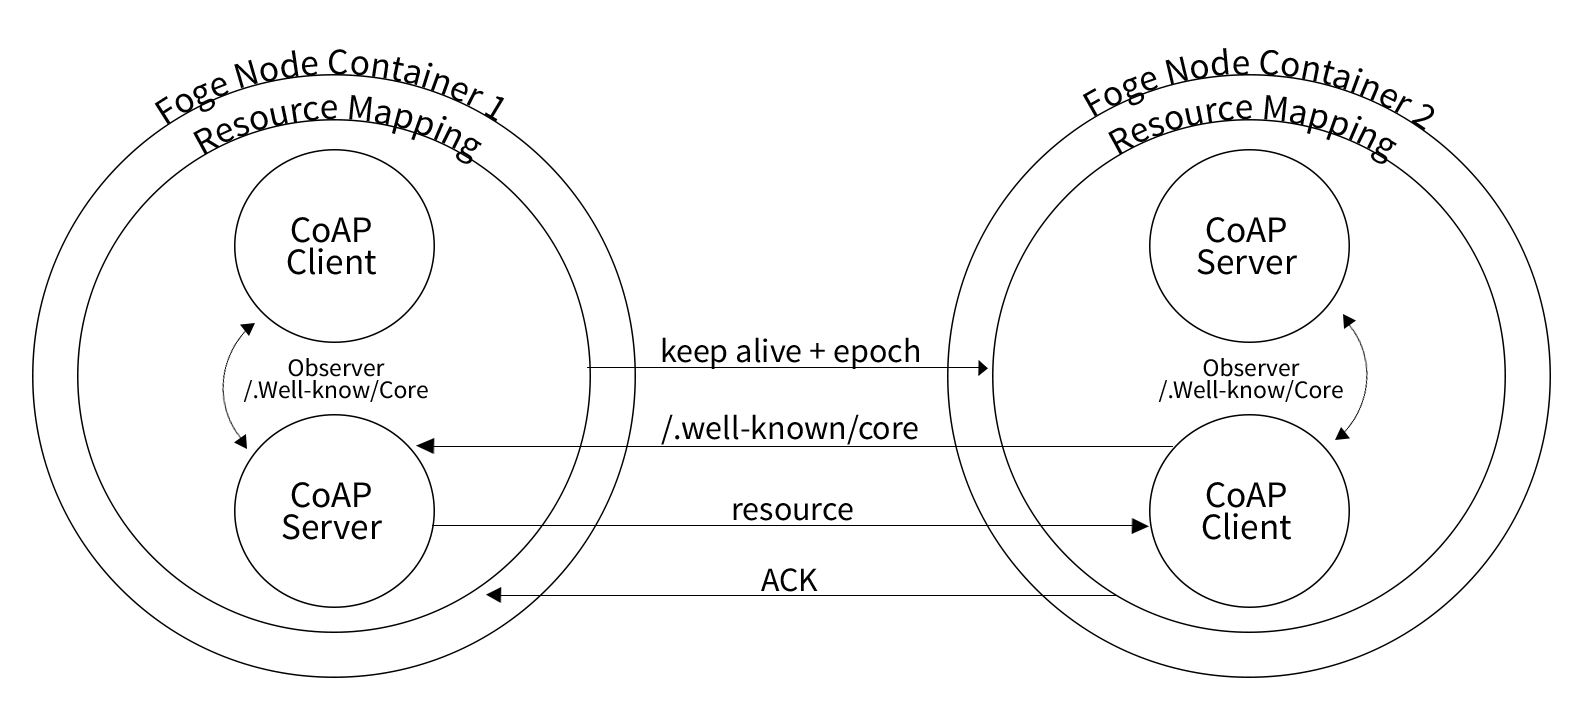
\includegraphics[width=.8\textwidth]{fig13.png}
    \caption [Fog node container]
    {\label{fig:fig13} Fog node container.}
\end{figure}


Além do protocolo de mapeamento em sí, este trabalho dispõe de uma API para o gerenciamento de recursos providos pelos CoAP servers.
Esta API possui métodos para listagem, remoção e criação de recursos e deve ser executada a partir do host que gerencia os container.
Assim, conseguimos proporcionar o dinamismo que a névoa necessita para a realização de testes no comportamento do protocolo de sincronização.


\section{Cenários de teste}
% Seção: "Cenários de teste"

Utilizando como base a Figura \ref{fig:fig7}, que retrata uma névoa com três fog nodes e seus respectivos edge devices, e partindo do pressuposto que todos os nodos da névoa já estão com seus recursos sincronizados corretamente,
iremos exemplificar os cenários de testes elencados abaixo.

\begin{enumerate}
    \item Entrada de algum equipamento na rede e este anunciando seus recursos. 
    \item Atualização das listas globais quando algum equipamento deixar de responder as mensagens de keep alive.
    \item Atualização da lista de recursos quando algum edge device é adicionado ou removido de um nodo da névoa.
\end{enumerate}

\begin{figure}[H]
    \centering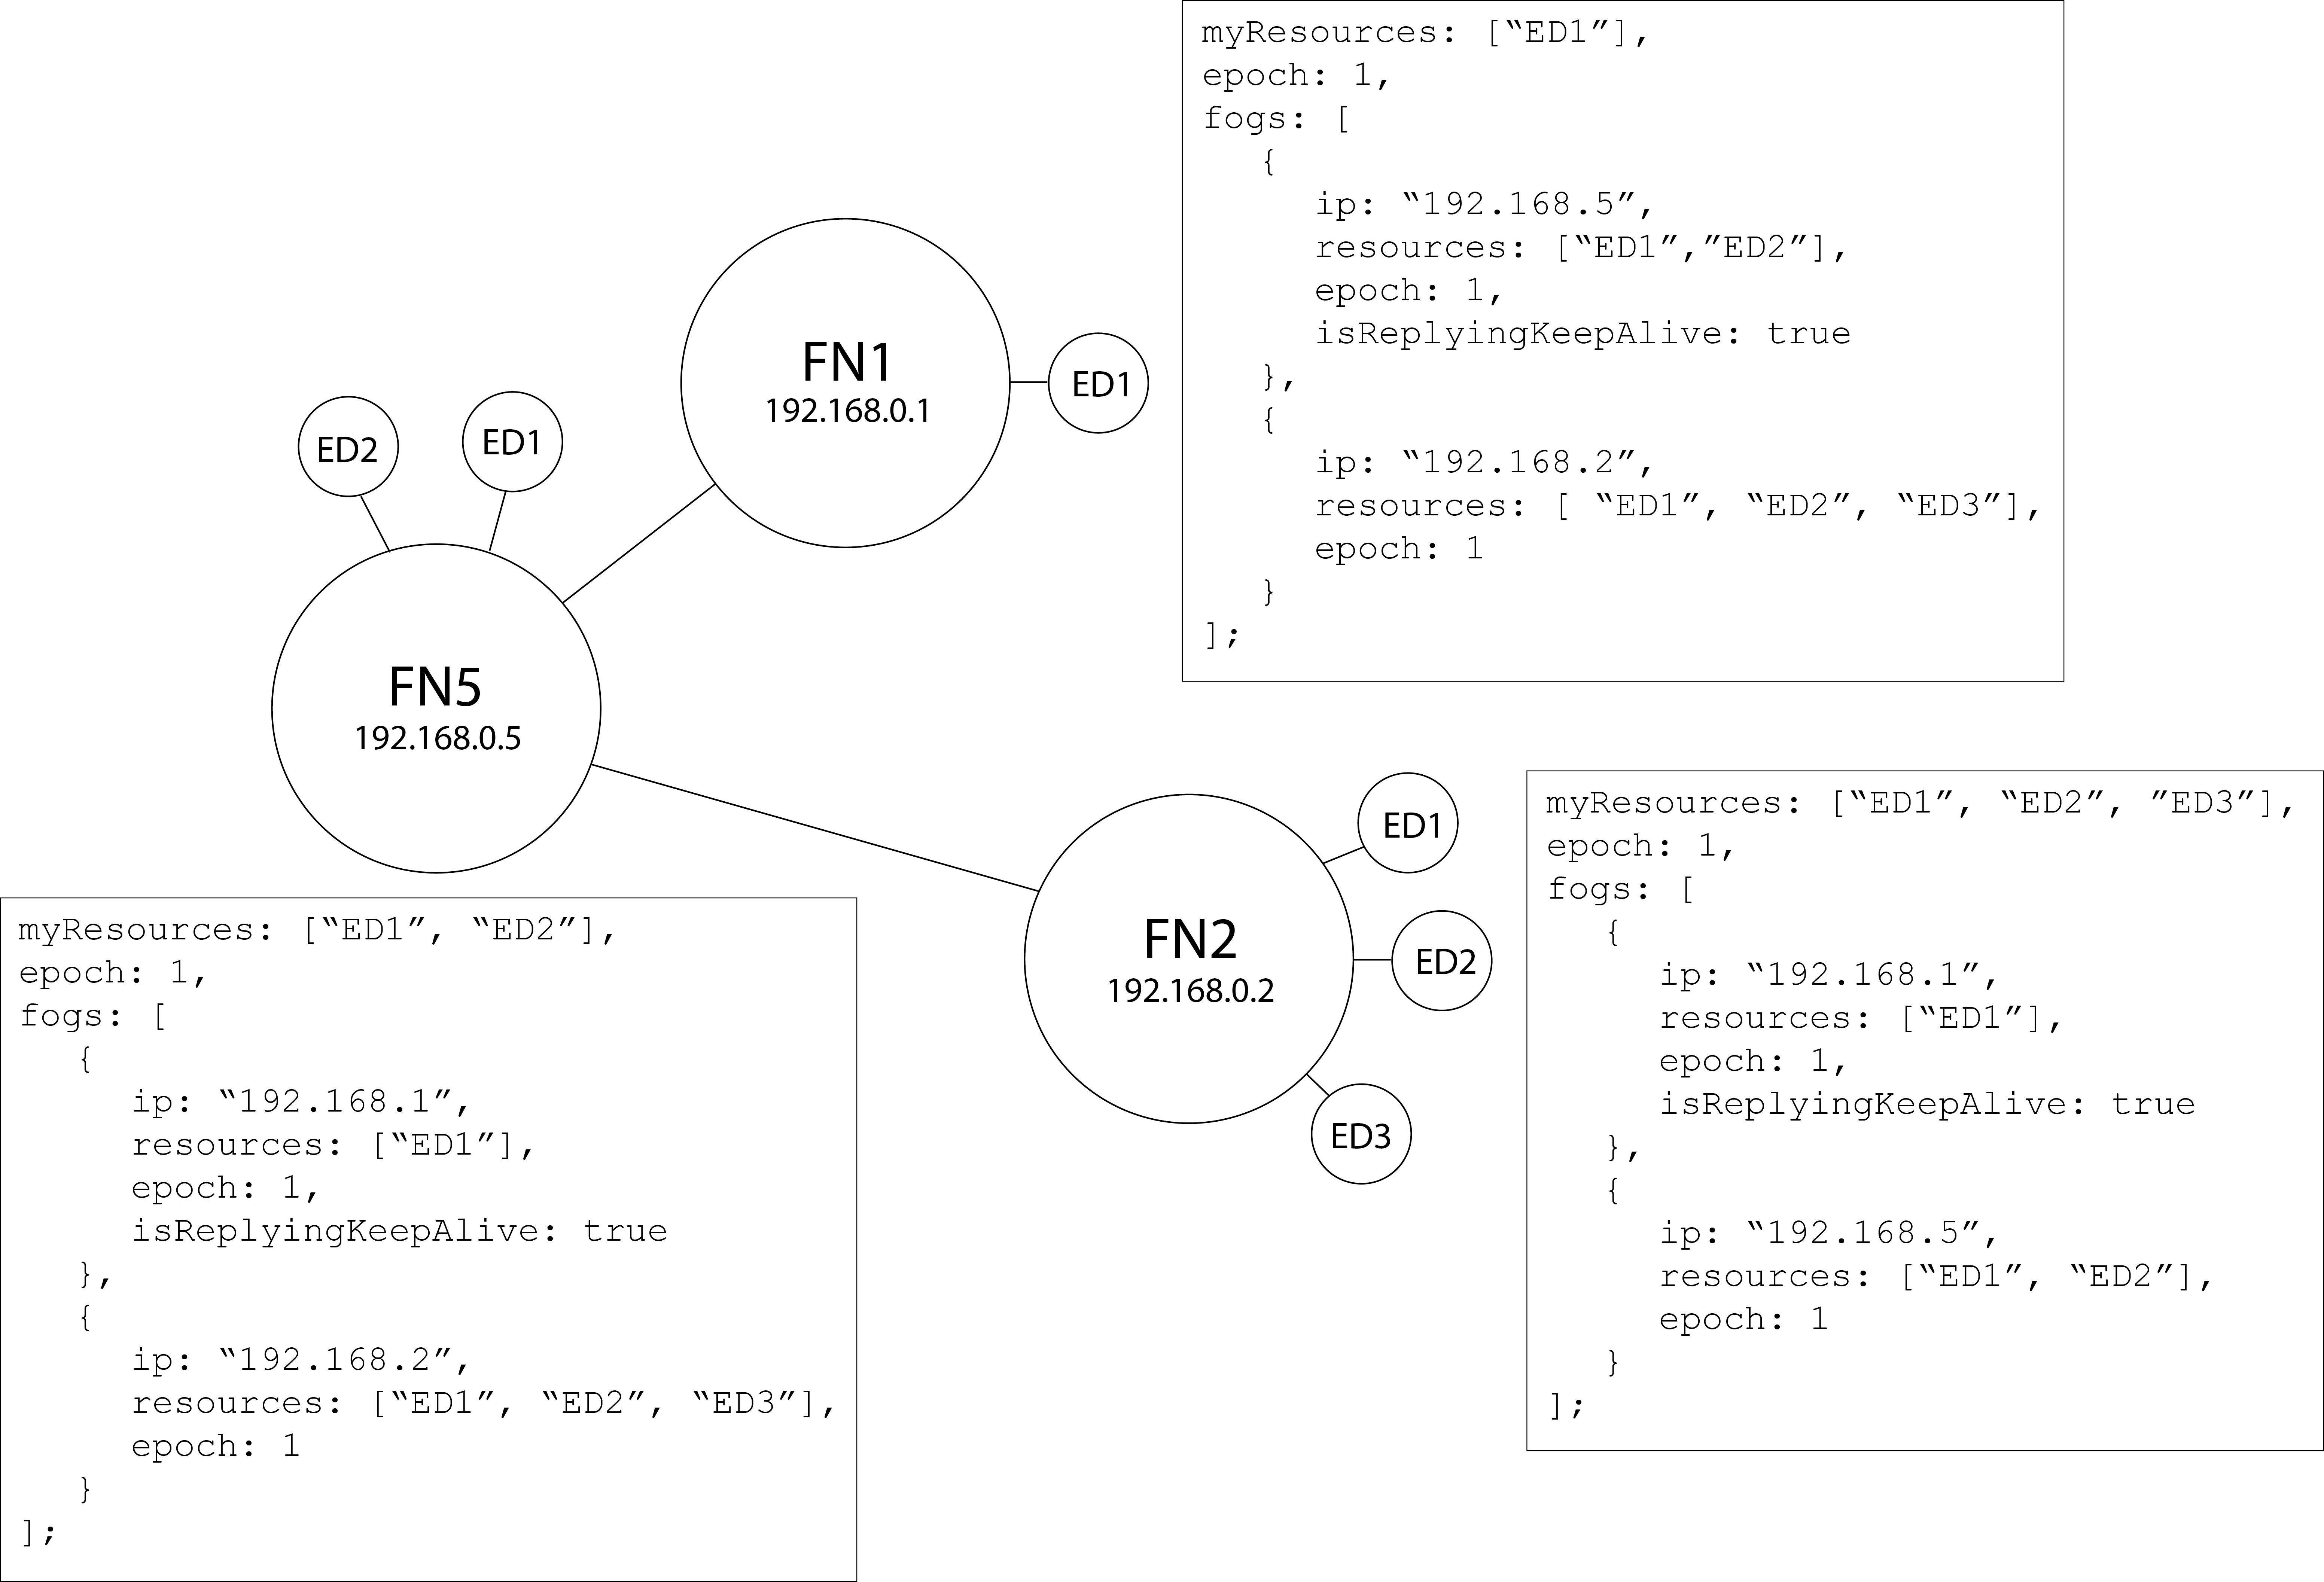
\includegraphics[width=.8\textwidth]{fig7.png}
    \caption[Topologia base para cenários de teste]
    {\label{fig:fig7} Topologia base para cenários de teste.}
\end{figure}

O primeiro item da listagem acima não será demonstrado agora, uma vez que as Subseções 3.3.1 e 3.3.2 já o fizeram, portanto, partiremos diretamente para o segundo item.

O segundo item trata-se de quando um nodo deixa de responder mensagens de keep alive, e a Figura \ref{fig:fig7} será utilizada para ilustrar esse funcionamento.
Na Figura \ref{fig:fig8}, que representa a continuação da Figura \ref{fig:fig7}, o nodo FN1 não respondeu no tempo previamente estipulado a mensagem de keep alive enviada pelo nodo FN2, 
portanto, o nodo destinatário foi marcado em FN2 como parcialmente inativo.


\begin{figure}[H]
    \centering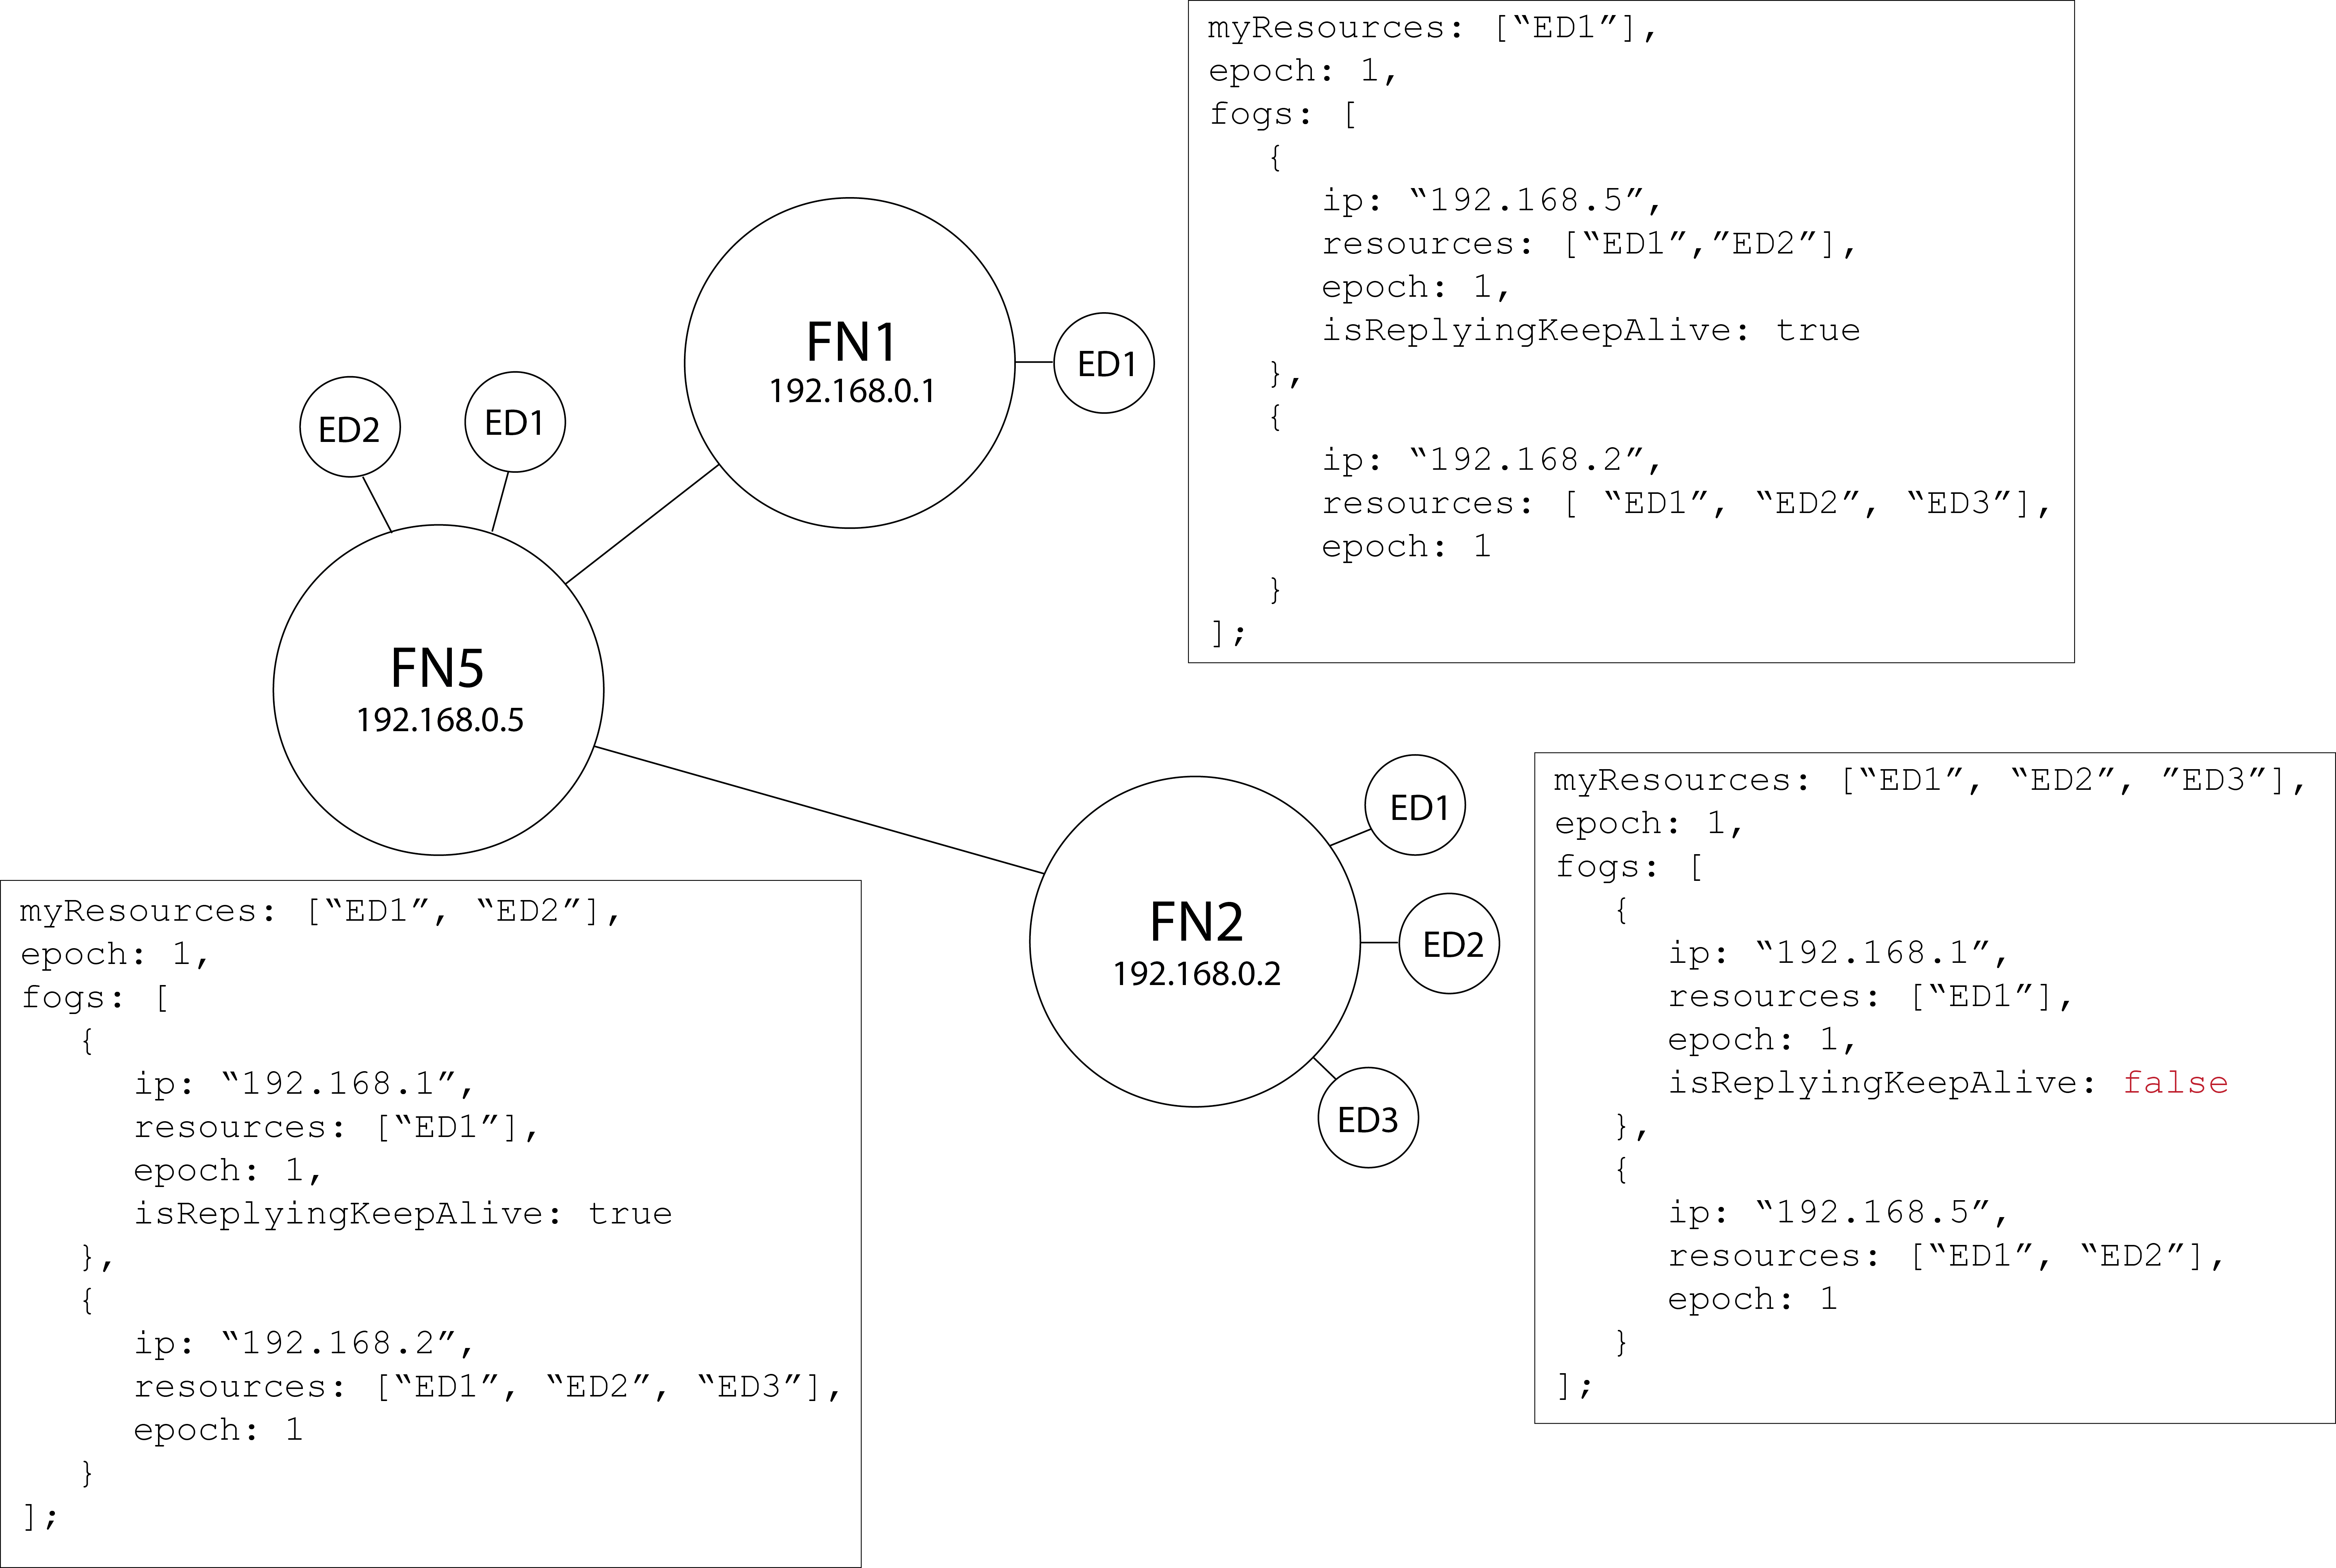
\includegraphics[width=.8\textwidth]{fig8.png}
    \caption [Nodo marcado como parcialmente inativo]
    {\label{fig:fig8} Nodo marcado como parcialmente inativo.}
\end{figure}

Já a Figura \ref{fig:fig9} representada como continuação da Figura \ref{fig:fig8}, demonstra que o nodo FN1 não respondeu novamente à mensagem de keep alive enviada por FN2, por isso, foi removido de sua lista de recursos. 

\begin{figure}[h!]
    \centering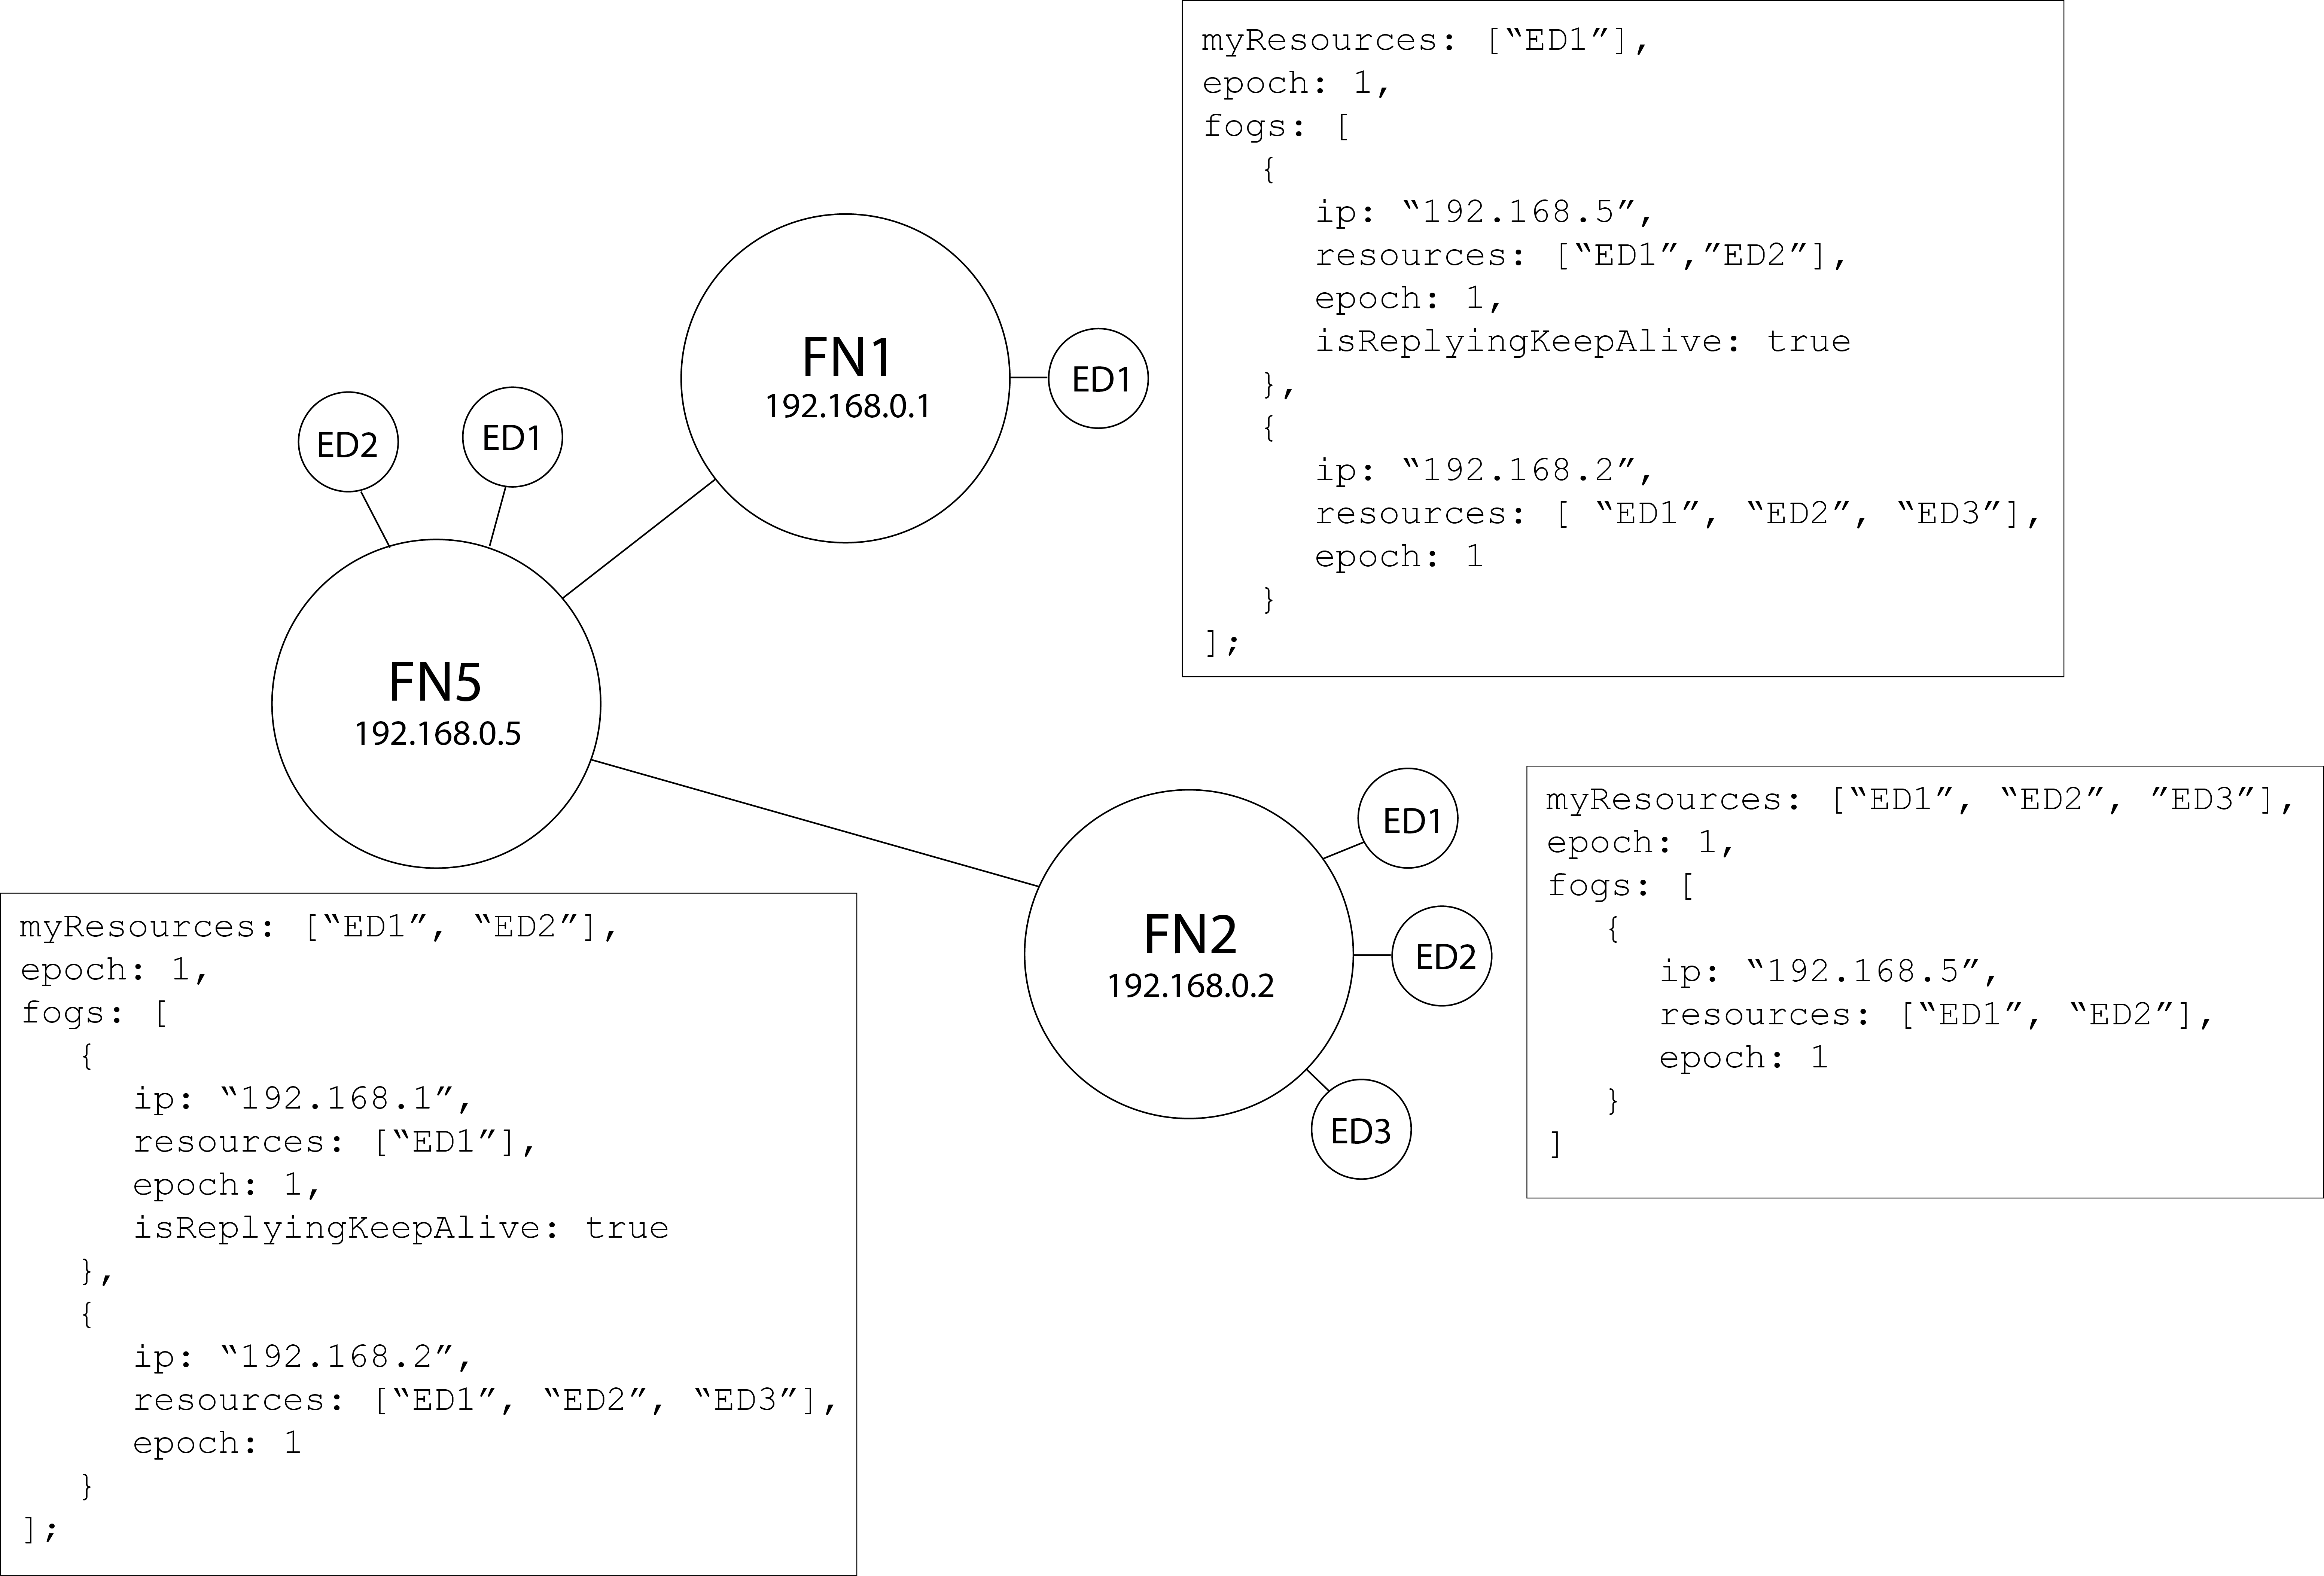
\includegraphics[width=.8\textwidth]{fig9.png}
    \caption [Nodo removido da lista de recursos]
    {\label{fig:fig9} Nodo removido da lista de recursos.}
\end{figure}

O terceiro item dos cenários de teste trata de quando o nodo está normalmente em operação, porém, um de seus recursos foi alterado, seja por incremendo de um novo edge device ou
pela remoção de um.

\begin{figure}[H]
    \centering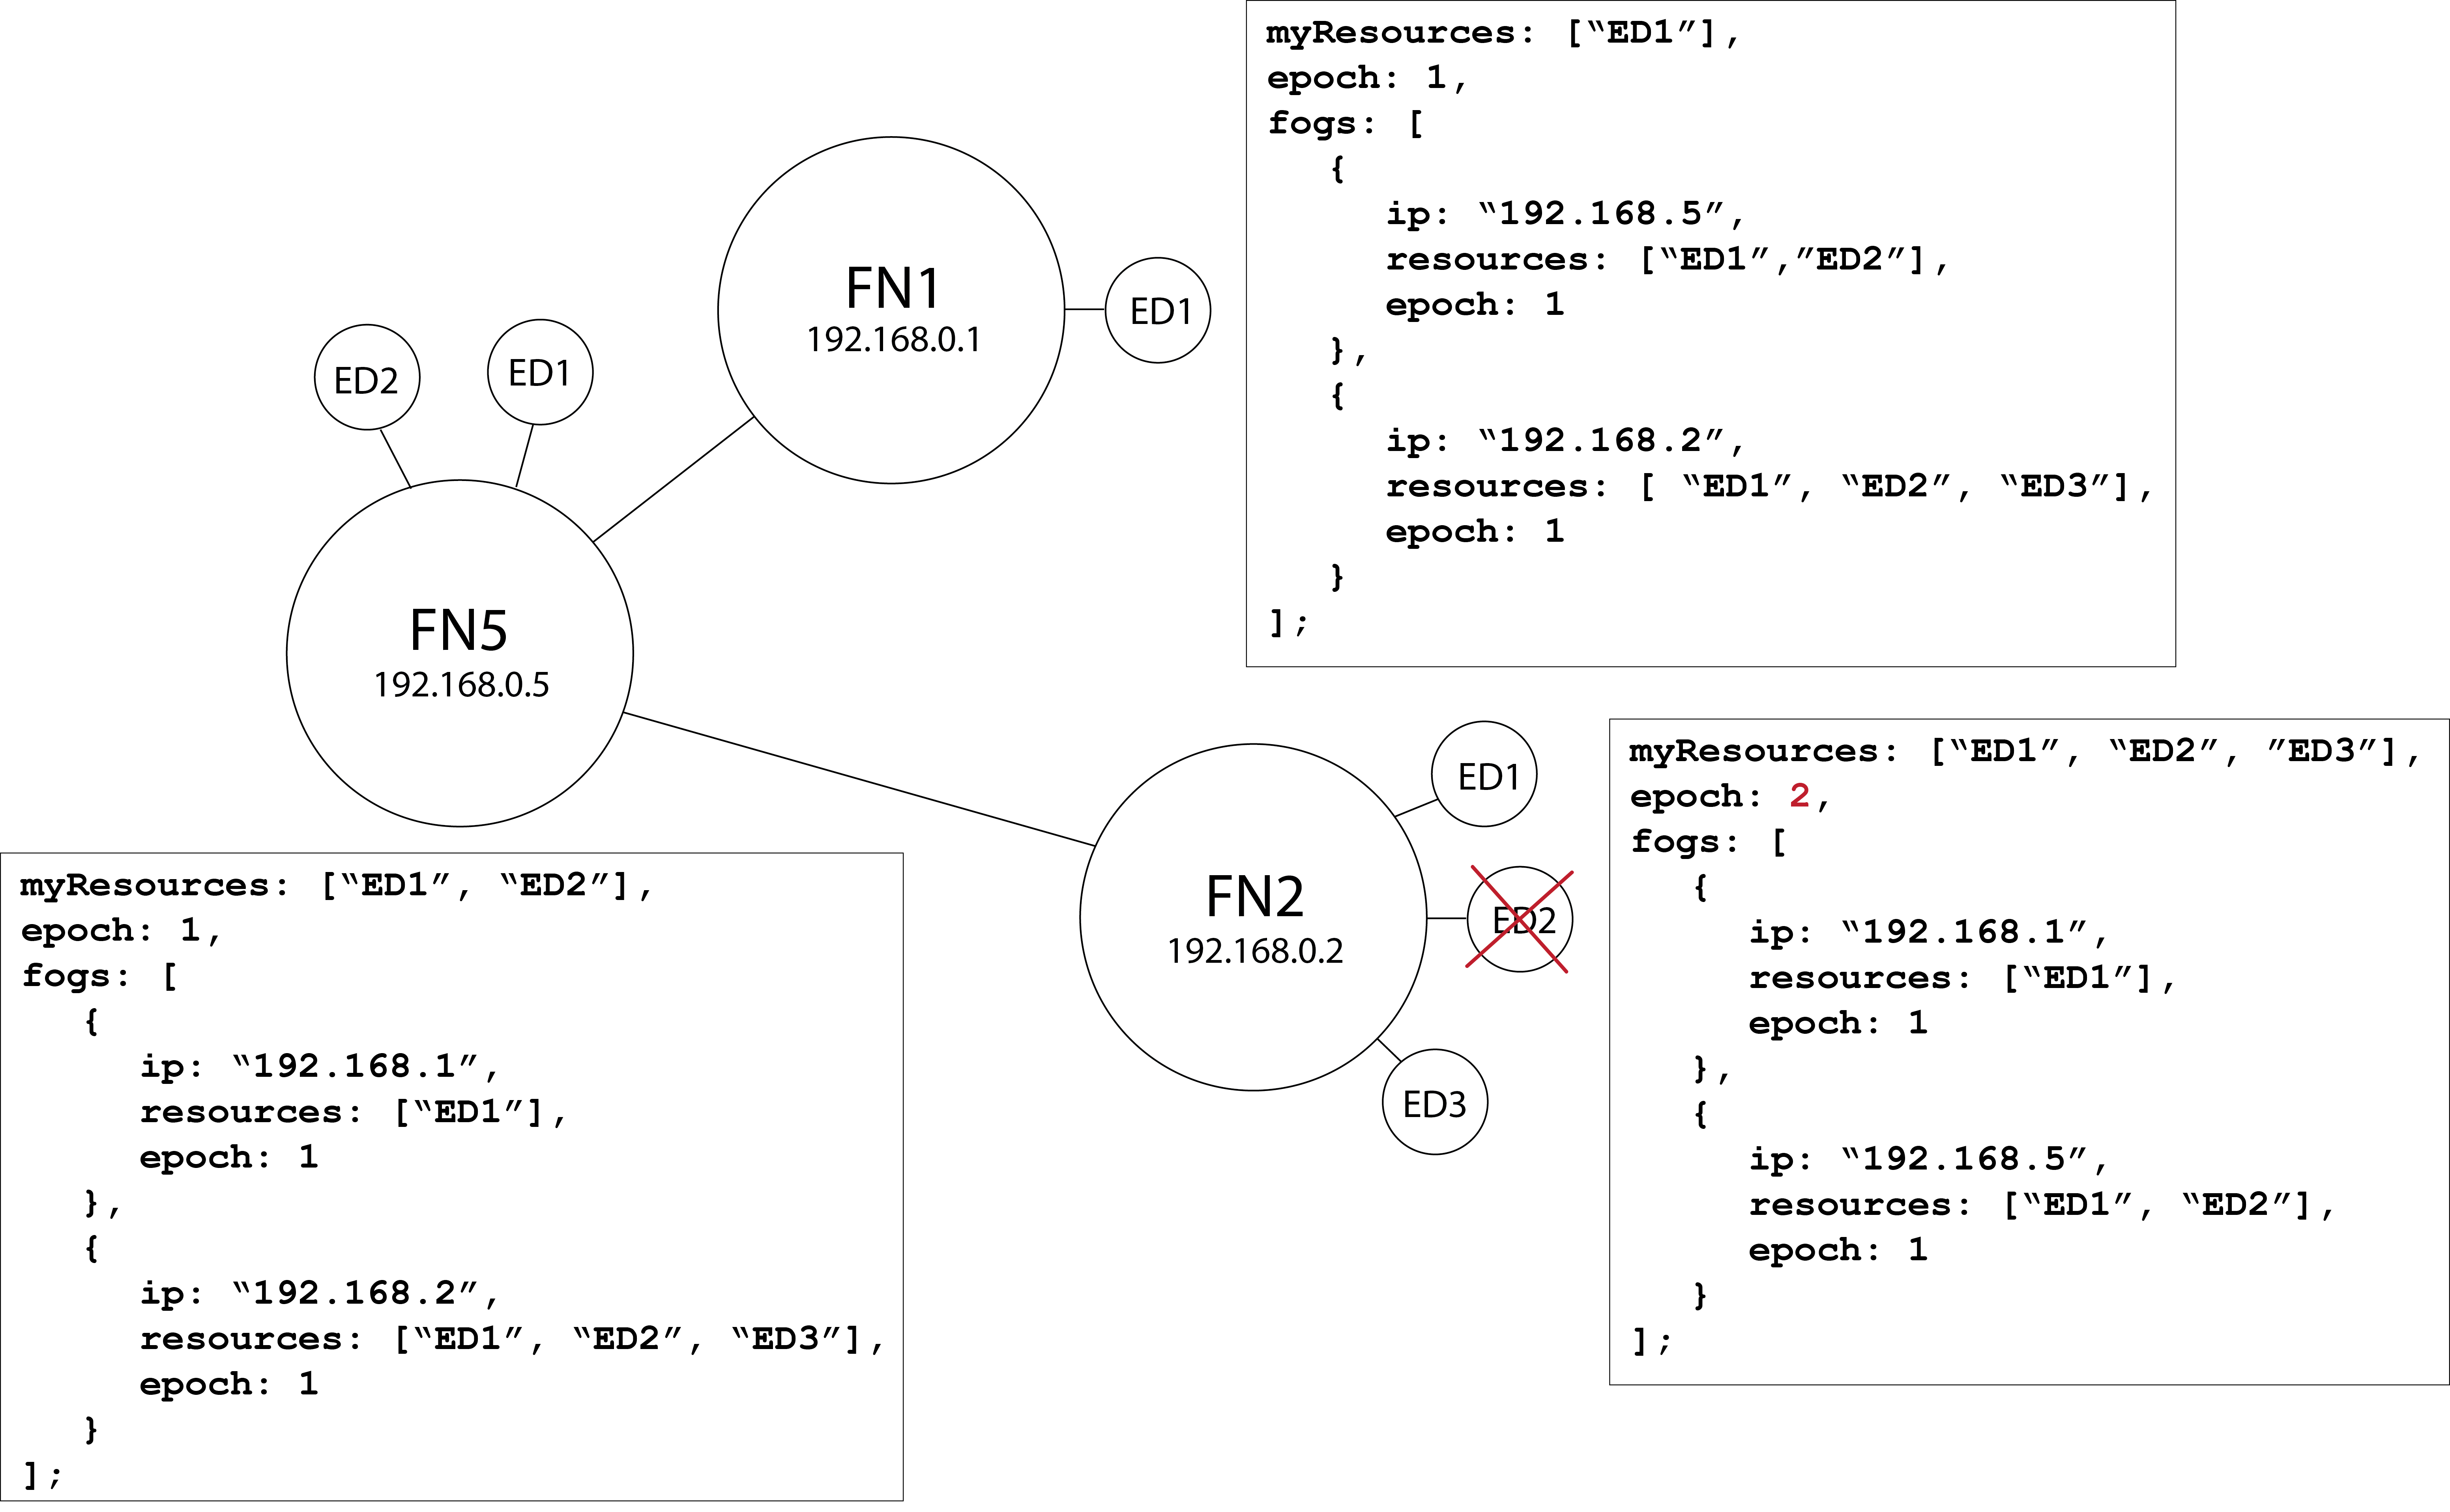
\includegraphics[width=.8\textwidth]{fig10.png} 
    \caption[Edge device fora de operação]
    {\label{fig:fig10} Edge device fora de operação.}
\end{figure}

Utilizaremos a Figura \ref{fig:fig10} como exemplo básico, e nela podemos observar que o edge device denominada ED2 vinculado ao nodo FN2 parou de funcionar.
Para este cenário, o nodo que hospeda ED2 deve estar ciente que este edge device está inoperante, e assim atualizar a sua \textit{época}.
O nodo que possui o edge device inoperante, então, terá sua época enviada juntamente com as mensagens de keep alive.
Assim, quando o nodo receber esta mensagem poderá comparar a época armazenada em sua lista de fogs com a época recebida pelo keep alive, e após a validação da divergencia realizará
um Requisição diretamente ao nodo para que possa atualizar sua lista de recursos globais.

\begin{figure}[H]
    \centering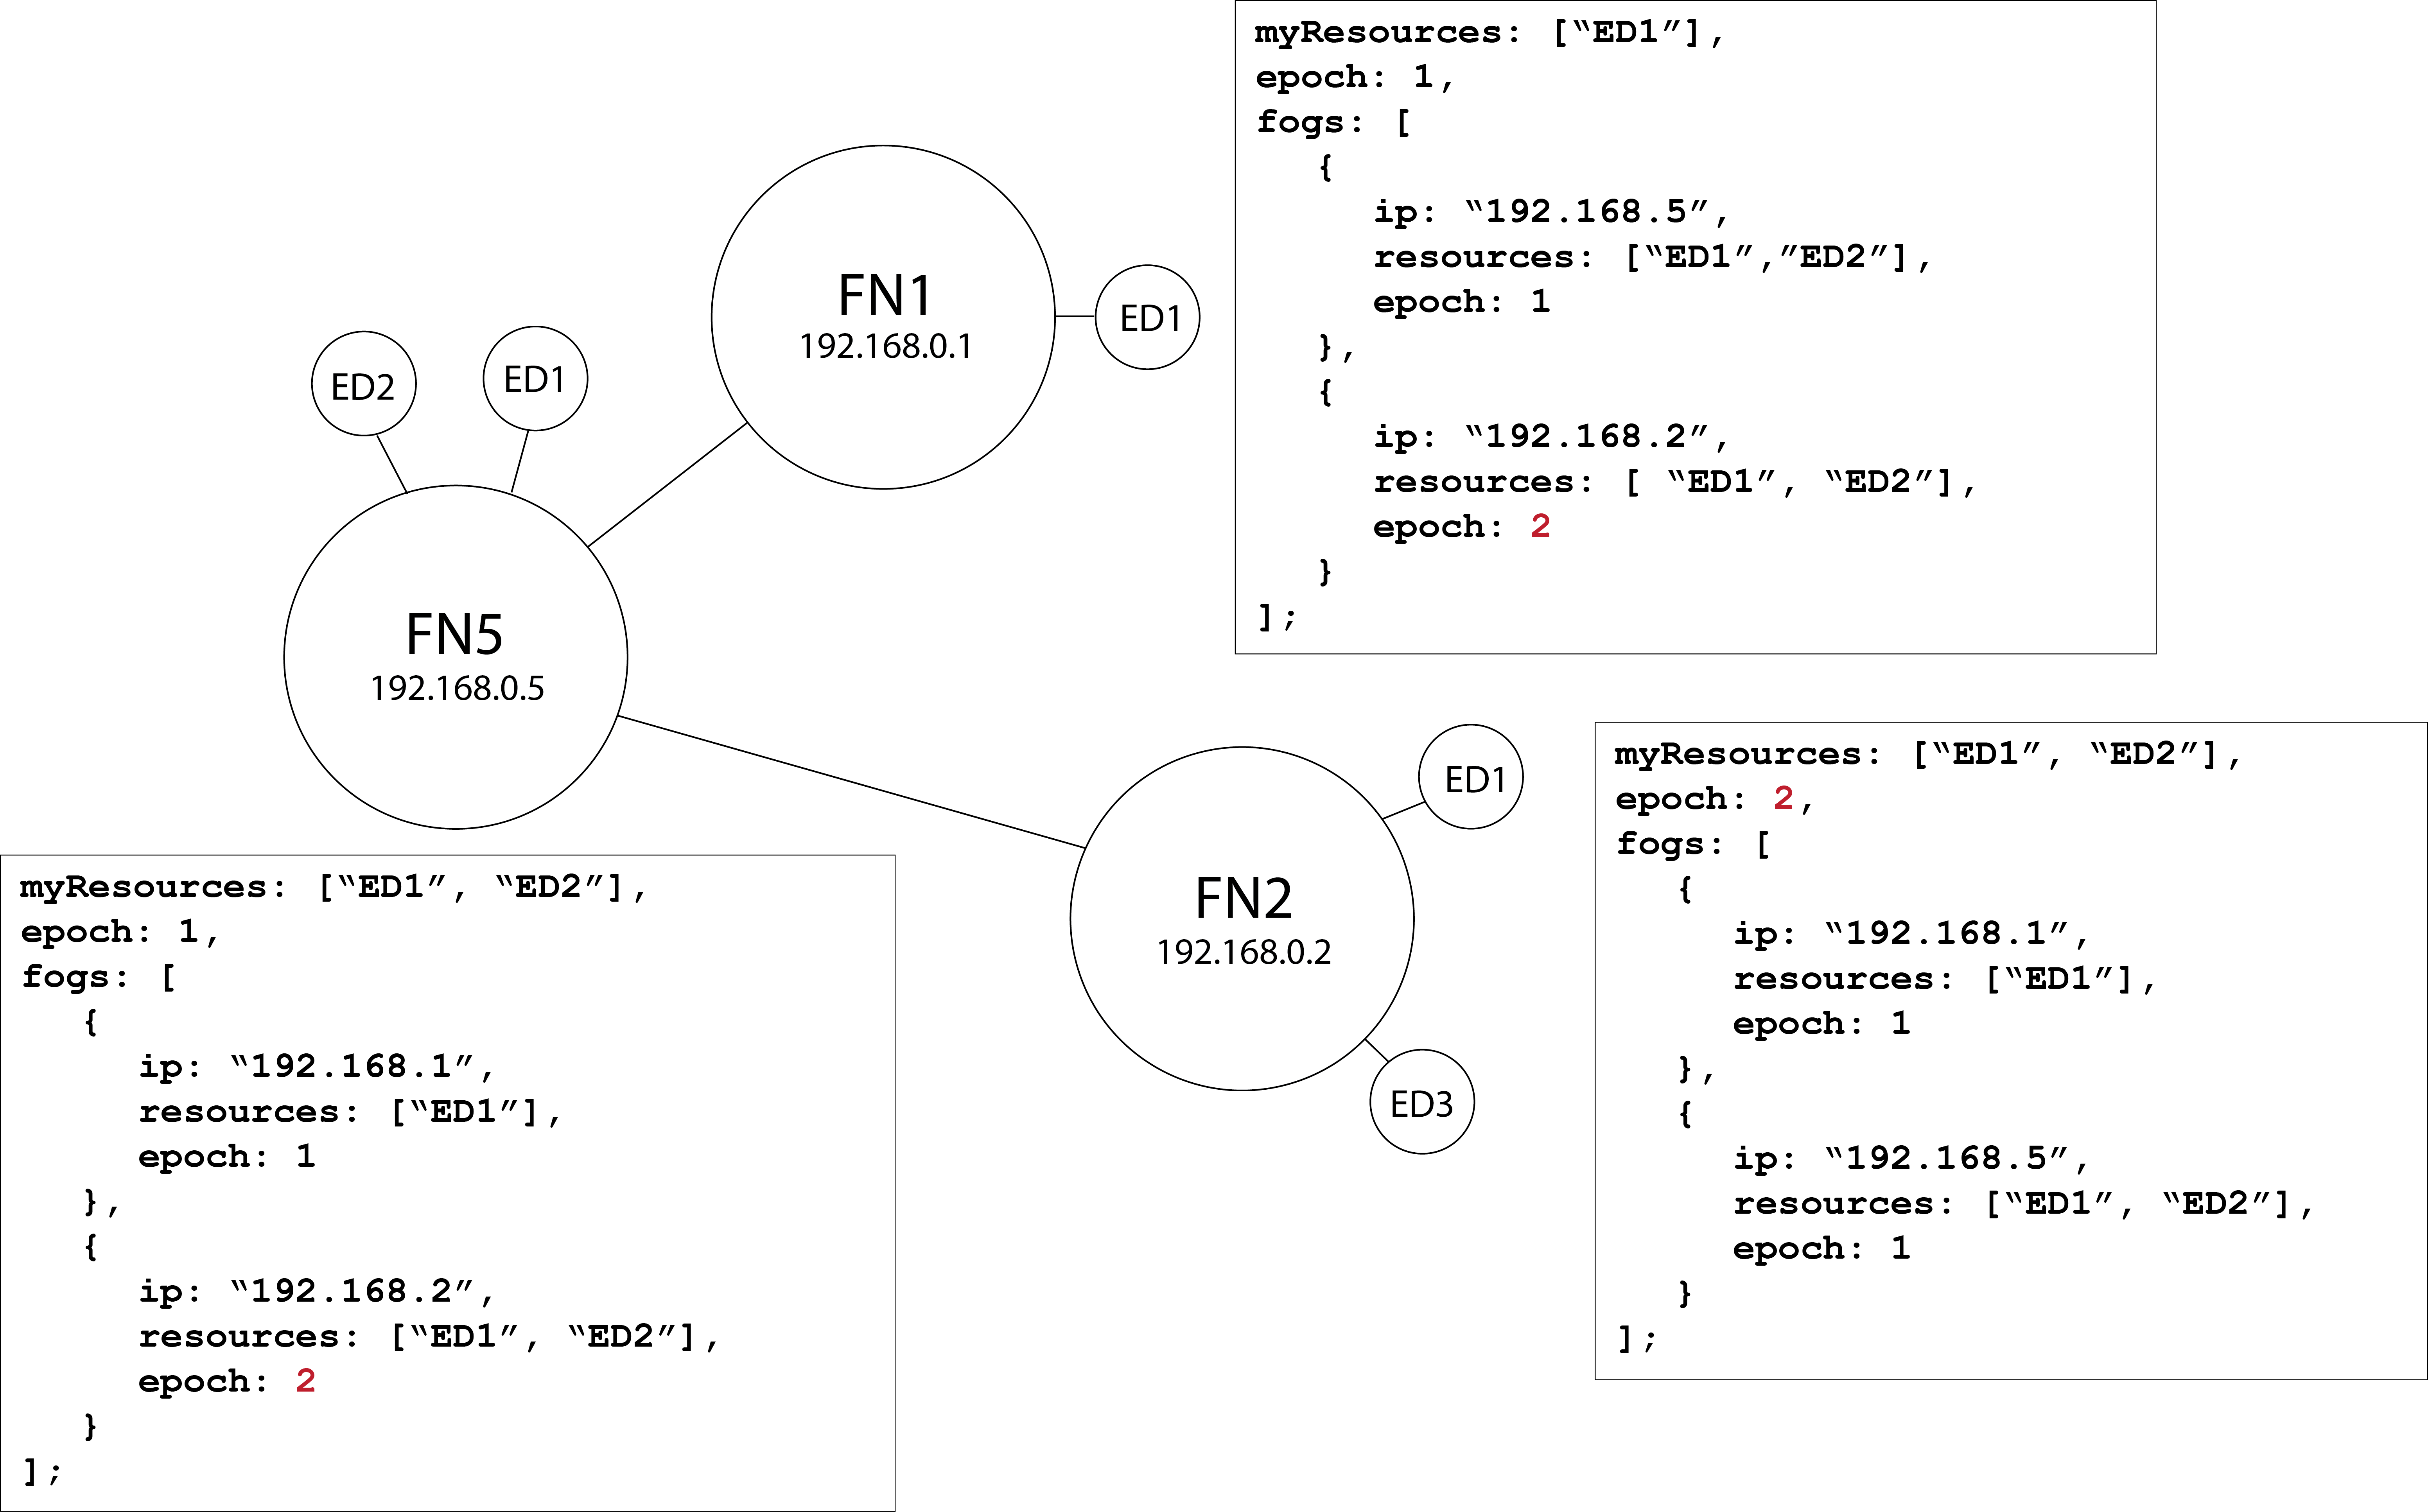
\includegraphics[width=.8\textwidth]{fig11.png} 
    \caption[Estado da névoa após atualização de recursos]
    {\label{fig:fig11} Estado da névoa após atualização de recursos.}
\end{figure}


\section{Estudos de caso}

As Subseções a seguir foram criadas com o intuito de ilustrar os testes previamente descritos, e para tal dois cenários serão propostos.

\subsection{Segurança residencial}

Como cenário para esse estudo de caso, podemos imaginar um bairro no qual os moradores estejam preucupados com a segurança de suas propriedades.
Partindo dessa suposição, as casas poderão contar com diversos atuadores tais como sensores de presença, câmeras de vigilância, luzes automatizadas, etc..
Em vista disso, cada casa pode ser considerada um fog node conectado a diversos edge devices.

Sabendo que o protocolo exposto atua no mapeamento e na sincronização de recursos, cada casa do bairro passa a dispor dessas funcioalidades.
Dessa maneira, as casas terão condições de monitorar eventos suspeitos que possam estar acontecendo nas redondezas.
Um exemplo de monitoramento está no uso das imagens captadas pelas câmeras de vigilância instaladas na casa A, mas acessados a partir da casa B.
Além disso, cada sensor adicionado ou removido estará, automaticamente, disponível a todos os fog nodes do bairro.


\subsection{Métricas no agronegócio}


Como cenário para esse estudo de caso, podemos imaginar uma fazenda que faz criação porcos.
Nessa fazenda os animais se alimentam em coxos individuais que possuem sensores que captam a temperatura, o peso, e a idenficação do animal, bem como medem os níveis de comida e água
que são consumidos.

Quando o animal entra nesse ambiente, o fog node é ligado e seus sensores começam a atuar nas medições.
Enquanto isso, um fog node com conexão a internet é encarregado de coletar os dados, processá-los e enviá-los a um servidor de armazenamento na nuvem.
Por fim, com o objetivo de economizar energia elétrica, os fog nodes e os sensores são desligados quando os animais deixam o local de alimentação.
A Figura \ref{fig:fig17} ilustra o cenário previamente exposto. Os detalhes sobre depuração são apresentados no Anexo A.


\begin{figure}[H]
    \centering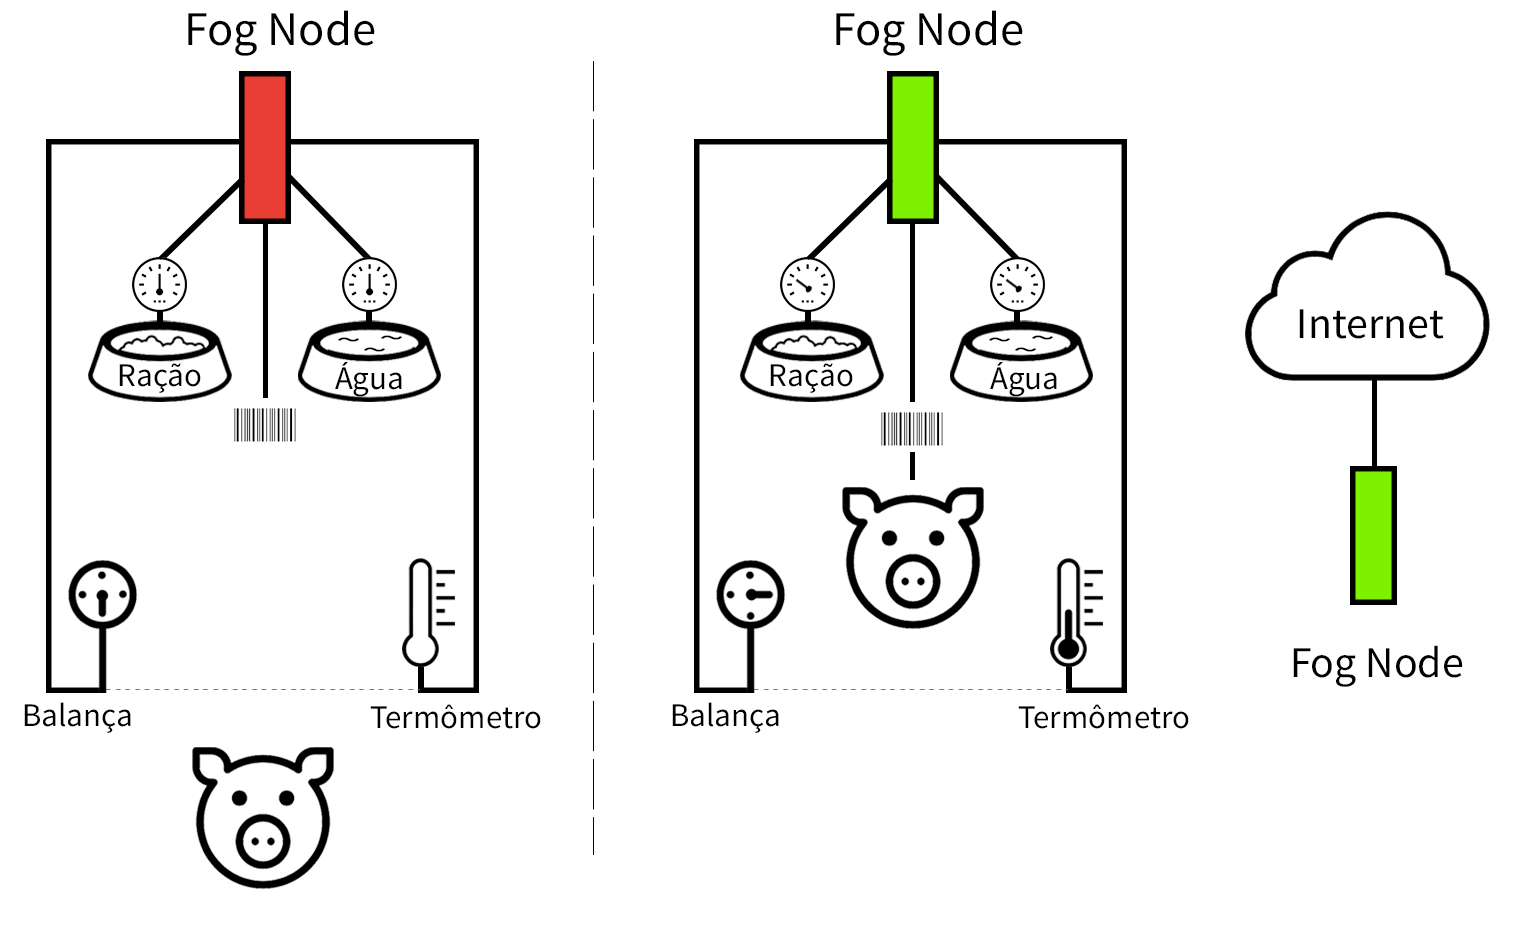
\includegraphics[width=.8\textwidth]{fig17.png} 
    \caption[ Métricas alimentares na criação de porcos]
    {\label{fig:fig17} Métricas alimentares na criação de porcos.}
\end{figure}